%%%%%%%%%%%%%%%%%%%%%%%%%%%%%%%%%%%%%%%%%%%%%%%%%%%%%%%%%%%%%%%%%%%%%%%%%%%
%                                                                         %
%                         Introduction to Scintillation                   %
%                                                                         %
%%%%%%%%%%%%%%%%%%%%%%%%%%%%%%%%%%%%%%%%%%%%%%%%%%%%%%%%%%%%%%%%%%%%%%%%%%%
Scintillation detectors (the detectors on which this work is based) utilize a scintillator to convert ionizing radiation into photons, and then transporting and capturing those the emitted photons, commonly with a photomultiplier tube (PMT).
The electrical signal from the PMT is then an indicator of a radiation event in the detector's scintillator material.
The current RPMs with \iso[3]{He} are ion chamber detectors, however, the proposed \iso[6]{Li} glass detectors and \iso[6]{LiF} doped ZnS:Ag detectors are scintillation based detectors. 

\subsection{Organic Scintillators}
An organic scintillator generally has a $\pi$-electron structure, as shown in \autoref{fig:pielectron}.
An incoming particle (generally electrons liberated from the energy deposition of the ionizing radiation) then excites one of the modes of the $\pi$-electron structure.
Higher singlet states rapidly (on the order of picoseconds) relax to the first singlet state, and excessive vibrational energy (populations of the vibrational sates) is lost.
Thus, after a short period of time the entire excitation population is in the $S_10$ state, and the decay of this state creates the prompt fluorescence.
\begin{figure}
  \centering
  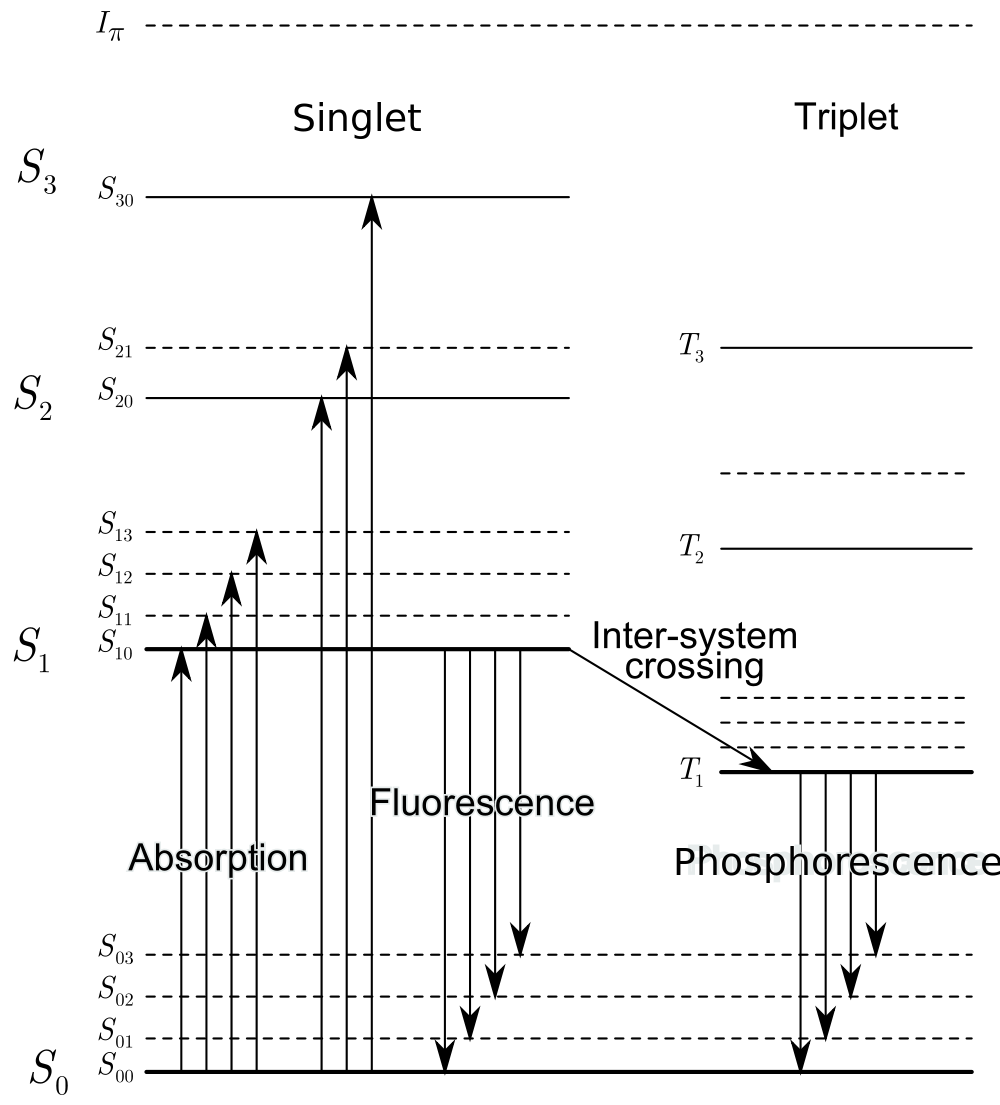
\includegraphics[width=\textwidth]{PiElectronSates}
  \caption[$\pi$ Electron Structure]{Typical $\pi$-electron structure of an organic molecule. The ground state of the molecule is shown as $S_0$, and excited single states are $S_1$, $S_2$ etc The triplet states are $T_1$, $T_2$, with the vibrational states as $S_OO$, $S_01$, $S_02$ and so forth. Figure from Wikipedia.}
  \label{fig:pielectron}
\end{figure}
The excitations of triplet states typically yield delayed scintillation events or phosphorescence.
An excited triplet states immediately decays to the $T_0$ state by internal degradation without a photon emission.
The $T_0$ state typically decays by interacting with another $T_0$ state in a $T_0 + T_0 \to S^* + S_0 + h\nu$ transition.
The excited singlet state $S^*$ then also decays to the $S_0$ state.
The $T_0 + T_0$ transitions is slower than direct singlet state de-excitations, and results in a slow component of the pulse, which can be used for pulse shape discrimination.

The light output of an organic scintillator can be empirically related to the energy deposition in the scintillator through the Birks equation.
In the absence of any quenching it is assumed that the light output per unit length is directly proportional to the energy deposition per unit length \eqref{eqn:LONoQuench}
\begin{align}
  \label{eqn:LONoQuench}
    \frac{dL}{dx} = S_B\frac{dE}{dx}
\end{align}
where \definevar{$S_B$}{absolute scintillation efficiency}.
If quenching of the light from molecules damaged by the radiation is also assumed to be proportional to the energy deposition per track length, than the Birks equation can be written as \eqref{eqn:BirksEquation}
\begin{align}
  \label{eqn:BirksEquation}
    \frac{dL}{dx} = \frac{S_B\frac{dE}{dx}}{1+kB\frac{dE}{dx}}
    \end{align}
    where \definevar{$S_B$}{absolute scintillation efficiency},\definevar{$\frac{dE}{dx}$}{linear stopping power} and \definevar{$kB$}{Birks parameter}, which accounts for the quenching of the light.
For low stopping powers (or particles with a very high energy) the light output per unit track length is linear as the quenching term can be neglected.
However, for particles with a large stopping power the light output along the track length becomes saturated by quenching.
This difference in the pulse height accounts for that difference in light output from a \SI{1}{\MeV} electron compared to a \SI{1}{\MeV} alpha.
The \textit{alpha to beta} ratio provides a measure of this effect, and for the GS20 glass is it typically around 0.23.
This effect is critical in the developed detectors are the reaction products of of the \iso[6]{Li} neutron absorption are both heavily charged particles subject to this effect.
Thus, while there is \SI{4.78}{\MeV} of reaction product energy released in the neutron absorption, the low alpha to beta ratio of the material limits the actual number of scintillation events.


Several factors need to be considered in order of a material to be considered as a scintillator:
\begin{itemize}
  \item The light yield should be linearly proportional to the energy deposition
  \item The material should be optically transparent to it's own wavelength of emission
  \item A short rise time with a fast decay time
\end{itemize}
Scintillators convert the energy deposited in the material by ionizing radiation in to photons.


